\documentclass[12pt, a4paper]{article}
\usepackage{amsmath}
\usepackage{amsfonts}
\usepackage{fontspec}
\usepackage{graphicx}
\usepackage{float}		%\begin{figure}[H] <- agrega el H
\usepackage{multirow}
\usepackage{multicol}
\usepackage{indentfirst}
\usepackage{caption} %comando \ContinuedFloat
\usepackage{array} %paquete para tabular
\usepackage{subcaption} %subfiguras y continuación de figura
\usepackage{pstricks-add}
\usepackage{bm}
\usepackage{enumitem} %cara utilizar distintos enumerate item
\usepackage{listings} %para poner codigos
\usepackage{esint} %permite usar integrales cerradas


\newcolumntype{P}[1]{>{\centering\arraybackslash}p{#1}} % P{} (mayúscula) en vez de p{} (minúscula)
\newcommand{\vect}[1]{\boldsymbol{#1}} %notación vector \vect{•}
\renewcommand{\contentsname}{Índice}
\renewcommand{\figurename}{Figura}
\renewcommand{\tablename}{Tabla}
\renewcommand\refname{Referencias}

%%% quita los ":" del \caption
\makeatletter
\long\def\@makecaption#1#2{%
\vskip\abovecaptionskip
\sbox\@tempboxa{#1. #2}%
\ifdim \wd\@tempboxa >\hsize
#1. #2\par
\else
\global \@minipagefalse
\hb@xt@\hsize{\hfil\box\@tempboxa\hfil}%
\fi
\vskip\belowcaptionskip}
\makeatother
%%%%%%%%%%%%%%%%%%%%%%%%%


\pagestyle{plain}


%FORMATO PÁGINA
%\hoffset
\voffset=-2cm
\oddsidemargin=0.8cm
%\evensidemargin
%\topmargin 		%entre sup y encab
%\headheight		%tamaño encabezado
%\headsep			%sep encab y text
\textheight=23cm		%altura texto
\textwidth=15cm		%ancho texto
%\marginparsep	%sep notmargen y text
%\marginparwidth	%ancho nota al marg
\footskip=1cm		%pie de pag
\setlength\parindent{0pt}	%sin identacion

\begin{document}

\thispagestyle{empty}

\hspace{-5mm}
\begin{minipage}[c]{7cm}
\centering

\includegraphics[width=4cm]{logoutfsm.jpg} \\
Universidad Técnica Federico Santa María
\end{minipage}
\hfill
\hspace{20mm}
\begin{minipage}[c]{7cm}
\centering

\includegraphics[width=4cm]{logomec1.jpg} \\
Departamento de Ingenieria Mecánica
\end{minipage}

\begin{center}
\vfill
 \Huge{{\bf Proyecto 2 }} \\ 
 \Huge{ {\bf Dinámica de fluidos computacional}} \\
\vfill
\end{center}

\vfill \hfill
\begin{tabular}{l @{ : } l}
Nombre &   Ignacio Apablaza \\
Rol & 201141007-6  \\
Profesores & Romain Gers \\
			& Olivier Skurtys \\
Asignatura & IPM468 \\
\end{tabular}

\newpage
%---------------------------------------------


\tableofcontents


\newpage
%---------------------------------------------

\section{Introducción}

Se estudia el perfil de velocidad de un flujo dentro de una tubería de sección circular. Se emplea el método de volúmenes finitos para la resolución numérica y se contrastan los resultados con los resultados analíticos. \\

En la Sección 2 se estudian los esquemas de discretización flujos convectivos y difusivos, además del esquema de integración temporal a utilizar en la implementación computacional, describiendose de manera general los pasos a seguir en la resolución de la ecuación de Navier-Stokes aplicado a un fluido newtoniano incompresible (Sección 3).\\

Para la integración temporal se emplea un esquema de Euler de orden 2 o esquema de Gear. Esta discretización permite integrar un intervalo de tiempo mediante el método de paso fraccionados o método ADI. En la Sección 4 se nombran algunas consideración al momento de discretizar el dominio físico, para lo cual se utilizan mallas desplazadas (\textit{staggered grid}).  Como se busca obtener un flujo completamente desarrollado se plantea condiciones de borde adecuadas para obtener estas características: Se emplean condición de presión conocida en la entrada y salida del tubo; y condición de periodicidad.\\

Los resultados númericos y teóricos se analizan en la Sección 5. Finalmente se realizan algunas observaciones en la Sección 6.


\newpage
%---------------------------------------------

%------------------------

\section{Discretización de las ecuaciones} \label{seccion2}

%------------------------

%ecuaciones gobernantes
\subsection{Ecuación de Navier Stokes discretizado}

La ecuación de conservación de la masa y de cantidad de movimiento para un fluido Newtoniano incompresible, despreciando los términos asociados al peso se pueden representar como:

\begin{equation}
\nabla \cdot \vect{v} = 0
\end{equation}

\begin{equation} \label{cdml}
\rho \dfrac{\partial \vect{v}}{ \partial t} + \rho \vect{v} \cdot \nabla \vect{v} = - \vec{\nabla} P + \nu \dfrac{ \partial^2 \vect{v} }{ \partial x^2 }
\end{equation}

La ecuación (\ref{cdml}) se expresa en forma adimensional. En coordenadas rectangulares se escribe:

\begin{equation}
\dfrac{\partial v_i^*}{\partial t^*} + v_j^* \dfrac{\partial v_i^*}{\partial x_j^*} = - \dfrac{\partial P^*}{\partial x_i^*} + \dfrac{1}{Re} \dfrac{\partial^2 v_i^*}{\partial x_j^* \, \partial x_j^*}
\end{equation}

Donde $v_i^*$, $P^*$, $x_j^*$ , $t^*$ representa a la variable adimensionadas respectivas. Para precindir de la notación ($^*$) se asume que todas las variables a utilizar están adimensionadas


%------------------------

%discretizacion espacial
%---------------------------------------------------

\subsection{Discretización espacial}

Ecuación de conservación/transporte de un escalar pasivo $\phi$:

\begin{equation} \label{transporte}
\dfrac{\partial \phi}{\partial t} + \nabla \cdot J = S_{\phi}
\end{equation}

donde $S_{\phi}$ representa el término fuente asociado a $\phi$ y $J$ a la contribución del flujo convectivo y difusivo:

\begin{equation}
J = \vect{v} \phi - \dfrac{1}{Re} \vec{\nabla} \phi
\end{equation}

Para obtener la formulación en volumenes finitos se aplica el método de residuos ponderados a la ecuación, con soporte compacto y utilizando el método de Galerkin [CITAR LIBRO]. Se recurre al teorema de valor medio representar la integral en función de terminos centrales. Sea $\phi_J$ un valor aproximado que caracteriza al escalar dentro del volumen de control $\Omega_{cv} = \Omega_J$. La ecuación discretizada resulta [CITAR LIBRO]:

\begin{equation}
\dfrac{\partial}{\partial t} \left( \phi_J \Omega_J \right) + \sum \left( F_i \, A_i \right)_J = \left( S_{\phi} \right)_J
\end{equation} 

Donde $F_i$ corresponde la contribución del flujo convectivo y difusivo en la cara $A_i$.
\begin{equation}
F = \underbrace{H(\phi)_C}_{\vect{v} \phi} + \underbrace{G(\phi)_D}_{-\vec{\nabla} \phi / Re}
\end{equation}

%---------------------------------------------------

\subsubsection{Término convectivo}

La discretización del término convectivo viene dado por
\begin{equation}
\iiint\limits_{\Omega} H(\phi) \, dV = \iiint\limits_{\Omega} \nabla \cdot \left( \vect{v} \phi \right) \, dV = \iint\limits_{\partial \Omega} \vect{v} \phi \cdot \vect{n} \, dA
\end{equation}

Aplicando el método de volumenes finitos resulta la siguiente expresión:

\begin{equation}
\iint\limits_{\partial \Omega} \vect{v} \phi \cdot \vect{n} \, dA \approx \left[ (\phi u)_e -(\phi u)_w \right] \Delta y + \left[ (\phi v)_n -(\phi v)_s \right] \Delta x
\end{equation}

Donde,

\begin{equation}
\begin{split}
&(u)_e = \frac{1}{2}(u_E+u_P) \\
&(u)_w = \frac{1}{2}(u_P+u_W) \\
&(v)_n = \frac{1}{2}(v_N+v_P) \\
&(v)_s = \frac{1}{2}(v_P+v_S)
\end{split}
\end{equation}

\begin{equation}
\begin{split}
&(\phi)_e = \frac{1}{2}(\phi_E+\phi_P) \\
&(\phi)_w = \frac{1}{2}(\phi_P+\phi_W) \\
&(\phi)_n = \frac{1}{2}(\phi_N+\phi_P) \\
&(\phi)_s = \frac{1}{2}(\phi_P+\phi_S)
\end{split}
\end{equation}

Luego,

\begin{equation}
\begin{split}
\iiint\limits_{\Omega} H(\phi) \, dV \approx \left[ \dfrac{\phi_E+\phi_P}{2} \dfrac{u_E+u_P}{2} - \dfrac{\phi_P+\phi_W}{2} \dfrac{u_P+u_W}{2} \right] \Delta y \\
+ \left[ \dfrac{\phi_N+\phi_P}{2} \dfrac{v_N+v_P}{2} - \dfrac{\phi_P+\phi_S}{2} \dfrac{v_P+v_S}{2} \right] \Delta x 
\end{split}
\end{equation}

Particularmente si se considera $\vect{H}(\vect{v}) = (h(u),h(v))$ se tiene que 

\begin{equation}
\begin{split}
h(u) \approx \underbrace{ \dfrac{1}{\Delta x} \left[ \dfrac{u_E+u_P}{2} \dfrac{u_E+u_P}{2} - \dfrac{u_P+u_W}{2} \dfrac{u_P+u_W}{2} \right]}_{\partial u^2 / \partial x} \, \Delta x \, \Delta y  \\
+ \underbrace{ \dfrac{1}{\Delta y} \left[ \dfrac{u_N+u_P}{2} \dfrac{v_N+v_P}{2} - \dfrac{u_P+u_S}{2} \dfrac{v_P+v_S}{2} \right] }_{\partial uv / \partial y} \, \Delta x \, \Delta y
\end{split}
\end{equation}

\begin{equation}
\begin{split}
h(v) \approx \underbrace{ \dfrac{1}{\Delta x} \left[ \dfrac{v_E+v_P}{2} \dfrac{u_E+u_P}{2} - \dfrac{v_P+v_W}{2} \dfrac{u_P+u_W}{2} \right]}_{\partial uv / \partial x} \, \Delta x \, \Delta y \\
+ \underbrace{ \dfrac{1}{\Delta y} \left[ \dfrac{v_N+v_P}{2} \dfrac{v_N+v_P}{2} - \dfrac{\phi_P+\phi_S}{2} \dfrac{v_P+v_S}{2} \right] }_{\partial v^2 / \partial y} \, \Delta x \, \Delta y
\end{split}
\end{equation}

	
%-------------------------------------------------

\subsubsection{Término difusivo}

Análogo a la discretización anterior, se aproxima el término difusivo utilizando el método de volúmenes finitos.

\begin{equation}
\iiint\limits_{\Omega} G(\phi) \, dV = \iiint\limits_{\Omega} \nabla \cdot \vec{\nabla} \phi \, dV = \iint\limits_{\partial \Omega} \vec{\nabla} \phi \cdot \vect{n} \, dA 
\end{equation}

Donde,

\begin{equation}
\iint\limits_{\partial \Omega} \vec{\nabla} \phi \cdot \vect{n} \, dA \approx \dfrac{1}{Re} \left[ (\vec{\nabla} \phi)_e - (\vec{\nabla} \phi)_w \right] \Delta y + \dfrac{1}{Re} \left[ (\vec{\nabla} \phi)_n - (\vec{\nabla} \phi)_s \right] \Delta x
\end{equation}

\begin{equation}
\begin{split}
&(\vec{\nabla} \phi)_e = \frac{1}{\Delta x}(\phi_E-\phi_P) \\
&(\vec{\nabla} \phi)_w = \frac{1}{\Delta x}(\phi_P-\phi_W) \\
&(\vec{\nabla} \phi)_n = \frac{1}{\Delta y}(\phi_N-\phi_P) \\
&(\vec{\nabla} \phi)_s = \frac{1}{\Delta y}(\phi_P-\phi_S)
\end{split}
\end{equation}

Reordenando los términos se obtiene:

\begin{equation}
\iiint\limits_{\Omega} G(\phi) \, dV \approx \dfrac{1}{Re} \dfrac{\Delta y}{\Delta x} \left[ \phi_E - 2\phi_P + \phi_w \right] + \dfrac{1}{Re} \dfrac{\Delta x}{\Delta y} \left[ \phi_N - 2\phi_P + \phi_S \right]
\end{equation}


%------------------------
\newpage
%---------------------------------------------

%------------------------

%discretización temporal
\section{Procedimiento computacional}

Se plantea un esquema BFD2 (\textit{Backward Differentiation Formula 2nd Order}). La derivada temporal $\partial \vect{v} / \partial t$ se aproxima mediante,

\begin{equation}
\dfrac{\partial \vect{v}}{\partial t} ^ {n+1} = \dfrac{3 \vect{v}^{n+1} -4\vect{v}^n + \vect{v}^{n-1}}{2 \Delta t} + \Theta(\Delta t^2) 
\end{equation}

El término convectivo en $t_{n+1}$ se obtiene por extrapolación de los términos en los instantes $t_{n}$ y $t_{n-1}$

\begin{equation}
H(\vect{v}^{n+1}) = 2 H(\vect{v}^n) - H(\vect{v}^{n-1})
\end{equation}

La ecuación a resolver mediante el método de volumenes finitos es:

\begin{equation} \label{ecuación_gobernante}
\dfrac{3 \vect{v}^{n+1} -4\vect{v}^n + \vect{v}^{n-1}}{2 \Delta t} + H(\vect{v}^{n+1}) = -\vec{\nabla} P + G(\vect{v}^{n+1})
\end{equation}



%------------------------

%predicción del campo de velocidad
\subsection{Predicción del campo de velocidad no solenoidal $\vect{v}^*$}

La resolución de (\ref{ecuación_gobernante}) requiere del cálculo de un predictor de la velocidad $\vect{v}$ dado por:

\begin{equation}
\dfrac{3 \vect{v}^{*} -4\vect{v}^n + \vect{v}^{n-1}}{2 \Delta t} + H(\vect{v}^{n+1}) = -\vec{\nabla} P + G(\vect{v}^{*})
\end{equation}

Sea $\vect{\delta V} = \vect{v}^* - \vect{v}^n $ y mediante una manipulación algebráica de la ecuación (\ref{ecuación_gobernante}) se obtiene una ecuación equivalente.

\begin{equation} \label{ecuación_gobernante_modificada}
\left( I - \dfrac{2 \Delta t}{3 \, Re} \Delta \right) \vect{\delta V} = \dfrac{\vect{v}^n-\vect{v}^{n-1}}{3} - \dfrac{2 \Delta t}{3} \left( 2 H(\vect{v}^n) - H(\vect{v}^{n-1}) + \vec{\nabla} P - G(\vect{v}^n) \right)
\end{equation} 

Aplicando el método ADI (\textit{Alternating Direction Implicit}) para descomponer al operador de Helmholtz ($I - \frac{2 \Delta t}{3 \, Re} \Delta $)

\begin{equation}
\left( I - \dfrac{2 \Delta t}{3 \, Re} \Delta \right) \approx \left( I - \dfrac{2 \Delta t}{3 \, Re} \dfrac{\partial^2}{\partial y^2} \right) \left( I - \dfrac{2 \Delta t}{3 \, Re} \dfrac{\partial^2}{\partial x^2} \right)
\end{equation}

Luego, resolver (\ref{ecuación_gobernante_modificada}) es equivalente de manera aproximada a resolver

\begin{equation}
\left( I - \dfrac{2 \Delta t}{3 \, Re} \dfrac{\partial^2}{\partial y^2} \right)  \left( I - \dfrac{2 \Delta t}{3 \, Re} \dfrac{\partial^2}{\partial x^2} \right) \delta V =  \dfrac{\vec{v}^n-\vec{v}^{n-1}}{3} - \dfrac{2 \Delta t}{3} \left( H(\vec{v}^{n+1}) + \vec{\nabla} P) \right)
\end{equation}

O bien,

\begin{align}
\left( I - \dfrac{2 \Delta t}{3 \, Re} \dfrac{\partial^2}{\partial x^2} \right) \delta \overline{V} &= RHS^n \label{primer_paso} \\ 
\left( I - \dfrac{2 \Delta t}{3 \, Re} \dfrac{\partial^2}{\partial y^2} \right) \delta V &= \overline{V} 
\end{align}

\subsubsection{Primer paso en la dirección $x$ ($\delta \overline{V}$)} 

Explicitando los términos de $RHS^n$ de la ecuación (\ref{primer_paso})

\begin{equation}
\left( I - \dfrac{2 \Delta t}{3 \, Re} \dfrac{\partial^2}{\partial x^2} \right) \delta \overline{V} = \dfrac{\vec{v}^n-\vec{v}^{n-1}}{3} - \dfrac{2 \Delta t}{3} \left( H(\vec{v}^{n+1}) + \vec{\nabla} P) \right) = RHS^n
\end{equation}

Recurriendo al método de residuos ponderados,

\begin{equation} 
\iiint_{\Omega} \Psi_i \left[ \left( I - \dfrac{2 \Delta t}{3 \, Re}  \dfrac{\partial^2}{\partial x^2} \right) \delta \overline{V}_i - RHS^n \right] \, dV = 0
\end{equation}

Y aplicando la formulación para volúmenes finitos, desarrrollando el primer término de la izquierda

\begin{equation}
\iiint_{\Omega_{cv}} \left( I - \dfrac{2 \Delta t}{3 \, Re}  \dfrac{\partial^2}{\partial x^2} \right) \delta \overline{V} \, dV =  \underbrace{\iiint_{\Omega_{cv}} \delta \overline{V} \, dV}_{(*)}  - \underbrace{\dfrac{2 \Delta t}{3 \, Re} \iiint_{\Omega_{cv}}  \dfrac{\partial^2 (\delta \overline{V}) }{\partial x^2} \, dV}_{(**)}
\end{equation}

Resolviendo $(*)$

\begin{equation}
\iiint_{\Omega_{cv}} \delta \overline{V} \, dV \approx  (\delta \overline{V})_P \, \Delta x \Delta y
\end{equation}

Resolviendo $(**)$

\begin{equation}
\dfrac{2 \Delta t}{3 \, Re} \iiint_{\Omega_{cv}}  \dfrac{\partial^2 (\delta \overline{V}) }{\partial x^2} \, dV \approx \dfrac{2 \, \Delta t}{3 \, Re} \dfrac{\Delta y}{\Delta x} \left( \delta \overline{V}_E -2 \delta \overline{V}_P + \delta \overline{V}_W \right)
\end{equation}

Reemplazando $(**)$ y $(***)$ en la (\ref{primer_paso}) se obtiene:

\begin{equation}
(\delta \overline{V})_P \, \Delta x \Delta y - \dfrac{2 \, \Delta t}{3 \, Re} \dfrac{\Delta y}{\Delta x} \left( \delta \overline{V}_E -2 \delta \overline{V}_P + \delta \overline{V}_W \right) = \iiint_{\Omega_{cv}} RHS^n \, dV
\end{equation}

El término $RHS^n$ se reemplaza por la ecuación la discretización planteada en la Sección \ref{seccion2} y por el campo de presión definido arbitrariamente a \textit{priori}. La ecuación anterior se traduce en resolver un sistemas de ecuaciones tridiagonal dado por,

\begin{equation}
\begin{split}
\left( - \dfrac{2 \, \Delta t}{3 \, Re} \dfrac{\Delta y}{\Delta x}  \right) \delta \overline{V}_E + \left( \Delta x \, \Delta y + \dfrac{4 \, \Delta t}{3 \, Re} \dfrac{\Delta y}{\Delta x}  \right) \delta \overline{V}_P + \left( - \dfrac{2 \, \Delta t}{3 \, Re} \dfrac{\Delta y}{\Delta x}  \right) \delta \overline{V}_W \\
 = \iiint_{\Omega_{cv}} RHS^n \, dV
\end{split}
\end{equation}

\subsubsection{Segundo paso en la dirección $y$ ($\delta V$)}

Se procede similar al paso anterior, con la diferencia de que no se recurre al método de volúmenes finitos, ya que se aplica sólo a un factor de la descomposición.  

\begin{equation}
(\delta \overline{V})_P - \dfrac{2 \, \Delta t}{3 \, Re} \dfrac{1}{(\Delta y)^2} \left( \delta V_E -2 \delta V_P + \delta V_W \right) = \delta \overline{V}_P
\end{equation}

Reeordenando los términos para obtener un sistema de ecuaciones tridiagonal

\begin{equation}
\begin{split}
\left( - \dfrac{2 \, \Delta t}{3 \, Re} \dfrac{1}{(\Delta y)^2}  \right) \delta V_E + \left( 1 + \dfrac{4 \, \Delta t}{3 \, Re} \dfrac{1}{(\Delta y)^2}  \right) \delta V_P + \left( - \dfrac{2 \, \Delta t}{3 \, Re} \dfrac{1}{(\Delta y)^2}  \right) \delta V_W \\
 = \delta \overline{V}_P
\end{split}
\end{equation}

Los pasos anteriores se realizan tanto para $u$ como para $v$ ya que $\vect{v}=\left\{ u,v \right\}^T$ y $\delta \vect{V} = \vect{v}^* - \vect{v}^n $. Cada paso de tiempo implica resolver 4 sistemas tridiagonales: 2 sistemas para la componente horizontal y 2 sistemas para la componente vertical de la velocidad. Finalmente se obtiene el predictor de la velocidad:

\begin{equation}
\vect{v}^* = \Big| \begin{matrix} u^* = u^n + \delta V_x \\ v^* = v^n + \delta V_y
\end{matrix}
\end{equation}



%------------------------

%correccion del campo de presión
%\subsection{Resolución de la ecuación de Poisson sobre la presión}

\begin{equation}
\Delta \phi = \dfrac{3}{2 \Delta t} \nabla \cdot \vec{v}^*
\end{equation}

\begin{equation}
\phi = \left( P^{n+1} - P^n \right) + \dfrac{1}{Re} \nabla \cdot \vec{v}^* 
\end{equation}

Nuevamente se aplica el método de residuos ponderados con formulación para volúmenes finitos.

\begin{equation}
\iiint_{\Omega} \Psi_i  \left[ \Delta \phi - \dfrac{3}{2 \Delta t} \nabla \cdot v_i^* \right] \, dV = 0
\end{equation}

Luego,

\begin{equation}
\iiint_{\Omega_J} \Delta \phi \, dV = \iiint_{\Omega_J} \dfrac{3}{2 \Delta t} \nabla \cdot v_i^* \, dV
\end{equation}

Recurriendo al teorema de Green-Ostrogradsky se rescribe la ecuación:

\begin{equation}
\iint_{\partial \Omega_J} \vec{\nabla} \phi \vec{n} \, dA = \dfrac{3}{2 \Delta t} \iint_{\partial \Omega_J} \vec{v}^* \cdot \vec{n} \, dA
\end{equation}

\paragraph{Discretización} La función auxiliar $\phi$ se discretiza en la malla desplazada asociada a la presión. Luego, los valores de los flujos de $\phi$ se aproximan en los bordes de cada volumen finito $\Omega_J$, mientras que los valores de las velocidad en $\partial \Omega_J$ son conocidos, sin necesidad de aproximarlos.

\begin{equation}
\begin{split}
\left[ \dfrac{\partial \phi}{\partial x} \Big|_e - \dfrac{\partial \phi}{\partial x} \Big|_w \right] \Delta y + \left[ \dfrac{\partial \phi}{\partial y} \Big|_n - \dfrac{\partial \phi}{\partial y} \Big|_s \right] \Delta x = \\ \dfrac{3}{2 \Delta t} \left( u^*_e - u_w^*  \right) + \dfrac{3}{2 \Delta t} \left( v^*_n - v_s^*  \right)
\end{split}
\end{equation}

Se discretizan las derivadas de $\phi$ implementando un esquemas CDS, obteniendose:

\begin{equation} \label{poisson_discreto}
\begin{split}
\left[ \dfrac{\phi_E-2\phi_P+\phi_W}{\Delta x} \right] \Delta y - \left[ \dfrac{\phi_N-2\phi_P+\phi_S}{\Delta y} \right] \Delta x = \\ \dfrac{3}{2 \Delta t} \left( u_e^* - u_w^* + v_n^* - v_s^* \right)
\end{split}  
\end{equation}

Agrupando los términos $\phi_{nb}$ resulta un sistema de ecuaciones lineales que en forma matricial se representa por una matriz pentadiagonal. Para resolverlo se utiliza el algoritmo TDMA (\textit{Tri-Diagonal MAtrix Algorithm}). Para ellos se define el término $B$ como,

\begin{equation}
B =  \dfrac{3}{2 \Delta t} \left( u_e^* - u_w^* + v_n^* - v_s^* \right)
\end{equation}

Se calcula un predictor (I):

\begin{equation}
\begin{split}
\left( \dfrac{\Delta y}{\Delta x} \right) \phi_E^I - \left( 2 \dfrac{\Delta y}{\Delta x} + 2 \dfrac{\Delta x}{\Delta y} \right) \phi_P^I + \left( \dfrac{\Delta y}{\Delta x} \right) \phi_W^I = \\ \left( \dfrac{\Delta x}{\Delta y} \right) \phi_N + \left( \dfrac{\Delta x}{\Delta y} \right) \phi_S + B
\end{split}
\end{equation}

Se calcula una corrección (II):

\begin{equation}
\begin{split}
\left( \dfrac{\Delta x}{\Delta y} \right) \phi_N^{II} - \left( 2 \dfrac{\Delta y}{\Delta x} + 2 \dfrac{\Delta x}{\Delta y} \right) \phi_P^{II} + \left( \dfrac{\Delta x}{\Delta y} \right) \phi_S^{II} = \\ \left( \dfrac{\Delta y}{\Delta x} \right) \phi_E^I + \left( \dfrac{\Delta y}{\Delta x} \right) \phi_W^I + B
\end{split}
\end{equation}

Un criterio de detención que suele utilizarse en establece lo siguiente: En cada punto de la malla se calcula un residuo $R$ como,

\begin{equation}
R = \sum a_{nb} \phi_{nb} + B - a_P \phi_P 
\end{equation}

La solución converge en la medida que $R$ tiende a cero. Más detalles del algoritmo se explican en \cite{patankar} y \cite{versteeg}. 



%------------------------

%correccion del campo de velocidad
%\subsection{Correción del campo de velocidad}

Una vez resuelto la ecuación de Poisson se procede a corregir la velocidad predicha en el primer paso:

\begin{equation}
\vec{v}^{n+1} = \vec{v} - \Delta t \nabla \phi
\end{equation}

Se recurre a la misma discretización utilizada en la ecuación (\ref{poisson_discreto}) para el campo auxiliar $\phi$.



%------------------------

%malla desplazada
%\section{Malla Desplazada (Staggered Grid)}

\subsection{Condiciones de contorno}
Se utilizan nodos ficticios para establecer las condiciones de frontera tipo Dirichlet o Neumann. Se utiliza la Figura \ref{fig1} como referencia.

\paragraph{Condiciones de Dirichlet} Utilizando una malla desplaza se observa que para ciertos bordes las condiciones se pueden implementar naturalemente. Sin embargo las condiciones de no deslizamiento en la pared superior no se pueden imponer directamente para $u$ (de la misma manera, en el lado izquierdo del borde no se pueden imponer directamente la condición de $v=0$) Para lograr ello se emplean nodos ficticios que sobresalen los contornos del dominio. Utilizando esquemas CDS se puede imponer que la velocidad $u$ en $\partial \Omega$ sea nulo

\begin{equation}
\dfrac{1}{2} (u + u_f) = 0 \rightarrow u_f = -u
\end{equation}

análogo para la componente vertical

\begin{equation}
\dfrac{1}{2} (v + v_f) = 0 \rightarrow v_f = -v
\end{equation}

El ejemplo se extiende a cualquier valor de velocidad $\vec{v} = \left\{ \overline{u}, \overline{v} \right\}$ en el contorno

\paragraph{Condiciones de Neumann} Se utiliza la misma lógica para imponer las condiciones de flujo en los contornos. Por ejemplo, para la variable $u$ se fija una condiciones de flujo nulo en los contornos y empleando un esquema CDS en el lado izquierdo se tiene:

\begin{equation}
\dfrac{\partial \hat{u}}{\partial x} \Big|_{\Gamma_u} \approx \dfrac{\hat{u}-\hat{u}_f}{\Delta x} = 0  \rightarrow  \hat{u}_f = \hat{u}
\end{equation}

\begin{figure} [H]
\centering
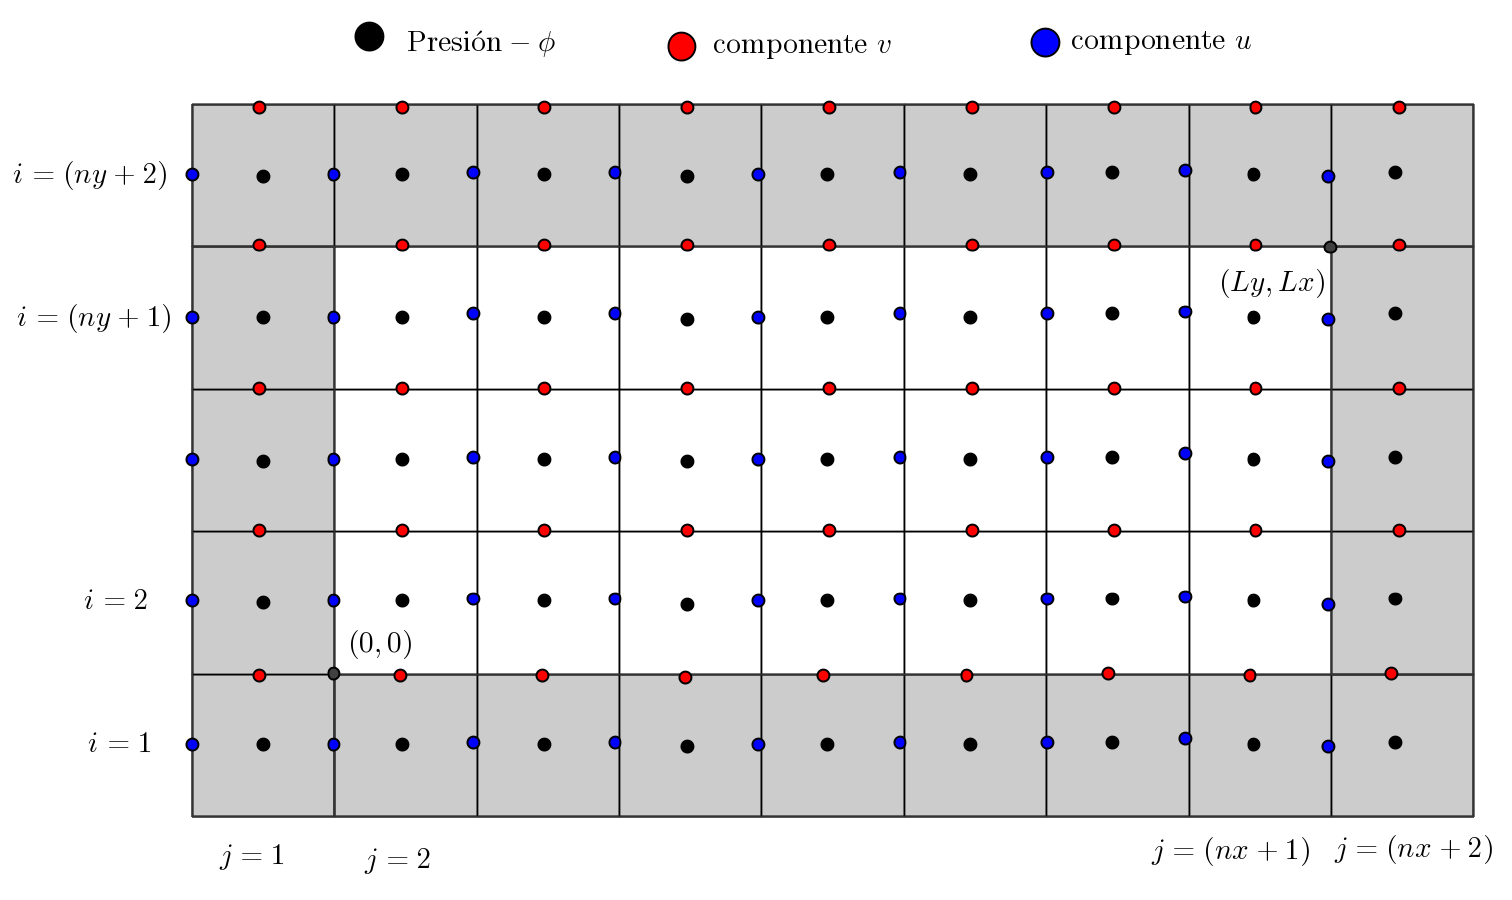
\includegraphics[width=0.8\textwidth]{malla.png}
\caption{Esquema representativo. Círculos azules: $u$ ; Rectángulos rojos: $v$ ; Equis : $P$} \label{fig1}
\end{figure}
\newpage
%---------------------------------------------

\section{ Descripción del problema }

El perfil parabólico de velocidad que resulta de un fluido que circula dentro de una tubería de sección circular se puede calcular analíticamente (Ley de Poiseuille). Este perfil se obtiene por la acción de los esfuerzos cortantes debido a la viscosidad del fluido. La ecuación que describe este perfil viene dada por:

\begin{equation}
u = \dfrac{\Delta P}{4 \mu L } \left( R^2 - r^2 \right)
\end{equation} 

donde $\Delta P$ es el gradiente de presión entre ambos extremos de la tubería, $\mu$ es la viscosidad dinámica, $L$ y $R$ corresponde a la longitud y al radio de la tubería, $r \in [0,R]$ es una posición dentro de la tubería.

\subsection{Dominio físico y numérico}

Se estudia el comportamiento de un fluido en tubería de radio $L_y$ y longitud $L_x$. Su modelo discretizado se representa mediante una malla regular desplazada (ver Figura \ref{malla}). Los puntos negros corresponden a las coordenadas de la presión (o de escalar pasivo $\phi$) y los puntos azules y rojos a las componentes horizontales y verticales de la velocidad, respectivamente. \\ 

Para facilitar el procedimiento de resolución, se incluyen nodos ficticios en la discretización, representados por los volúmenes de color ( $ i=1,ny+2 $ para $ j=1 $ y $j=nx+2$ ;  $ j=1,nx+2 $ para $ i=1 $ e $i=ny+2$ ) que contienen las condiciones de contorno del problema. Notar de la Figura que las variables $u(i,j=1)$ y $v(i=ny+2,j)$ no aportan información al problema, pero se conservan para respetar la nomenclatura de los puntos de la malla.

\begin{center}
\begin{figure}
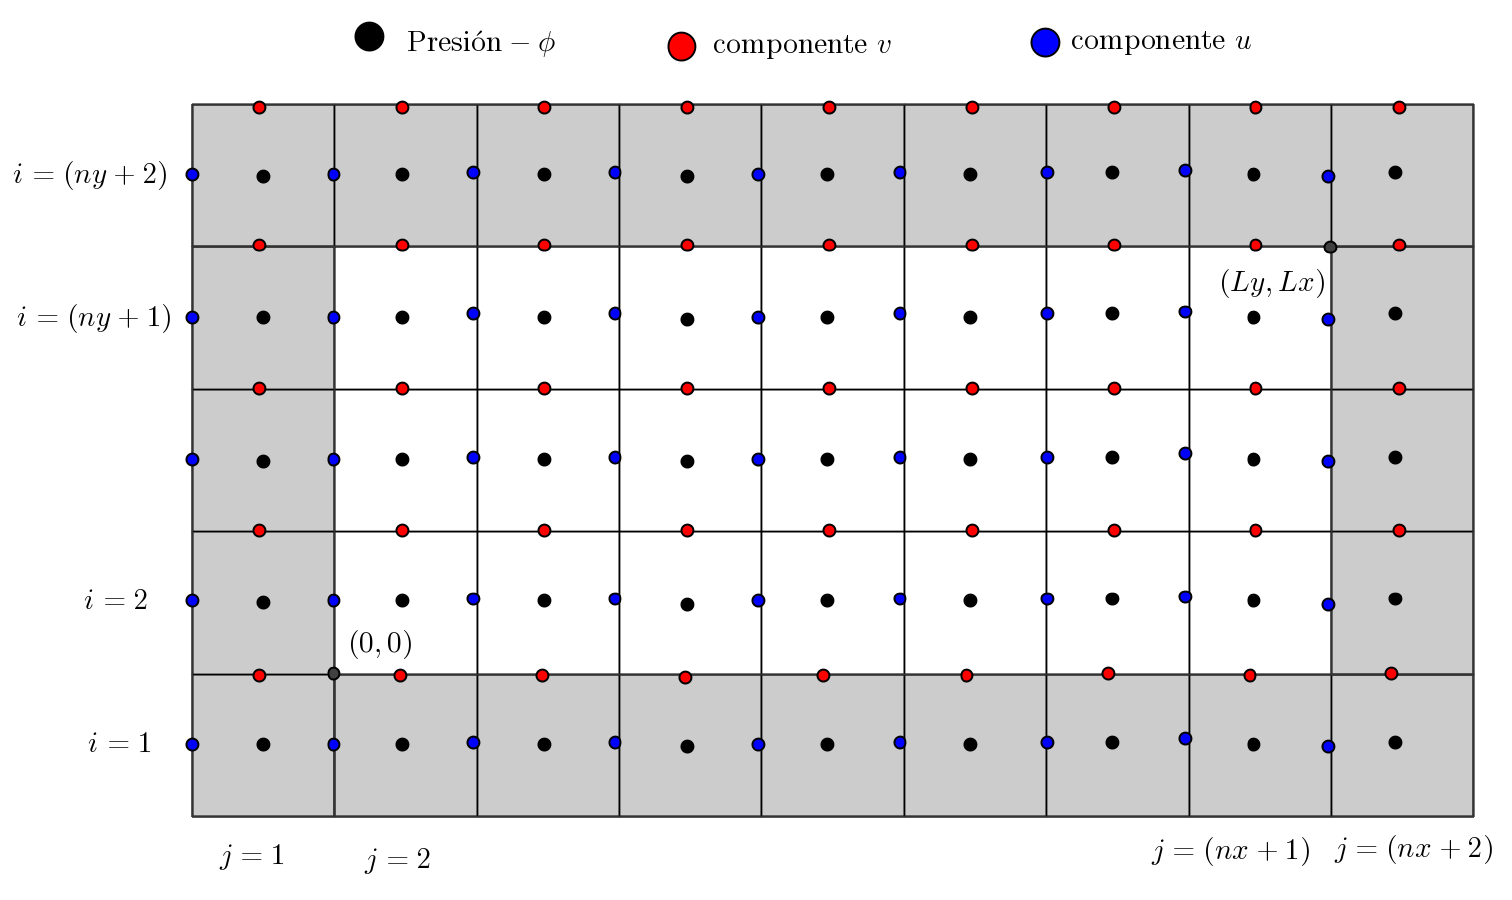
\includegraphics[width=1\textwidth]{malla.png}
\caption{Malla regular de discretización del dominio} \label{malla}
\end{figure}
\end{center}

\subsection{Algoritmo de resolución}

En la Figura \ref{algoritmo} se muestra un diagrama de flujo del código implementado. El preámbulo (dimensiones, número de nodos, parámetros físicos, etc.) está incluido de un módulo. 

\begin{enumerate}
\item Inicio programa \texttt{CFD\_POISEUILLE} (Preámbulo contenido en el módulo)
\item Se imponen las condiciones iniciales
\item Se imponene las condiciones de contorno
\item \label{iter} Inicio de la iteración de $k$ desde 1 a $nt$ ($nt$: número de pasos de tiempo)
\item \label{cor_vel} Se calcula la predicción de la velocidad
\item Se corrige la presión mediante la resolución de la ecuación de Poisson de $\phi$
\item Se verifica la convergencia de las variables. Si el término de fuente de masa o el número de iteraciones satisfacen cierto criterio, se regresa al paso \ref{cor_vel}. Caso contrario, continua con el siguiente paso
\item Se corrige el campo de velocidad
\item Se verifica si se logra un flujo estacionario. Si está en estado transiente, se imponen las condiciones de contorno y se vuelve al paso \ref{iter}. Caso contrario, se exportan los datos y se grafican.
\item Fin del programa \texttt{CFD\_POISEUILLE}
\end{enumerate}

\begin{center}
\begin{figure}
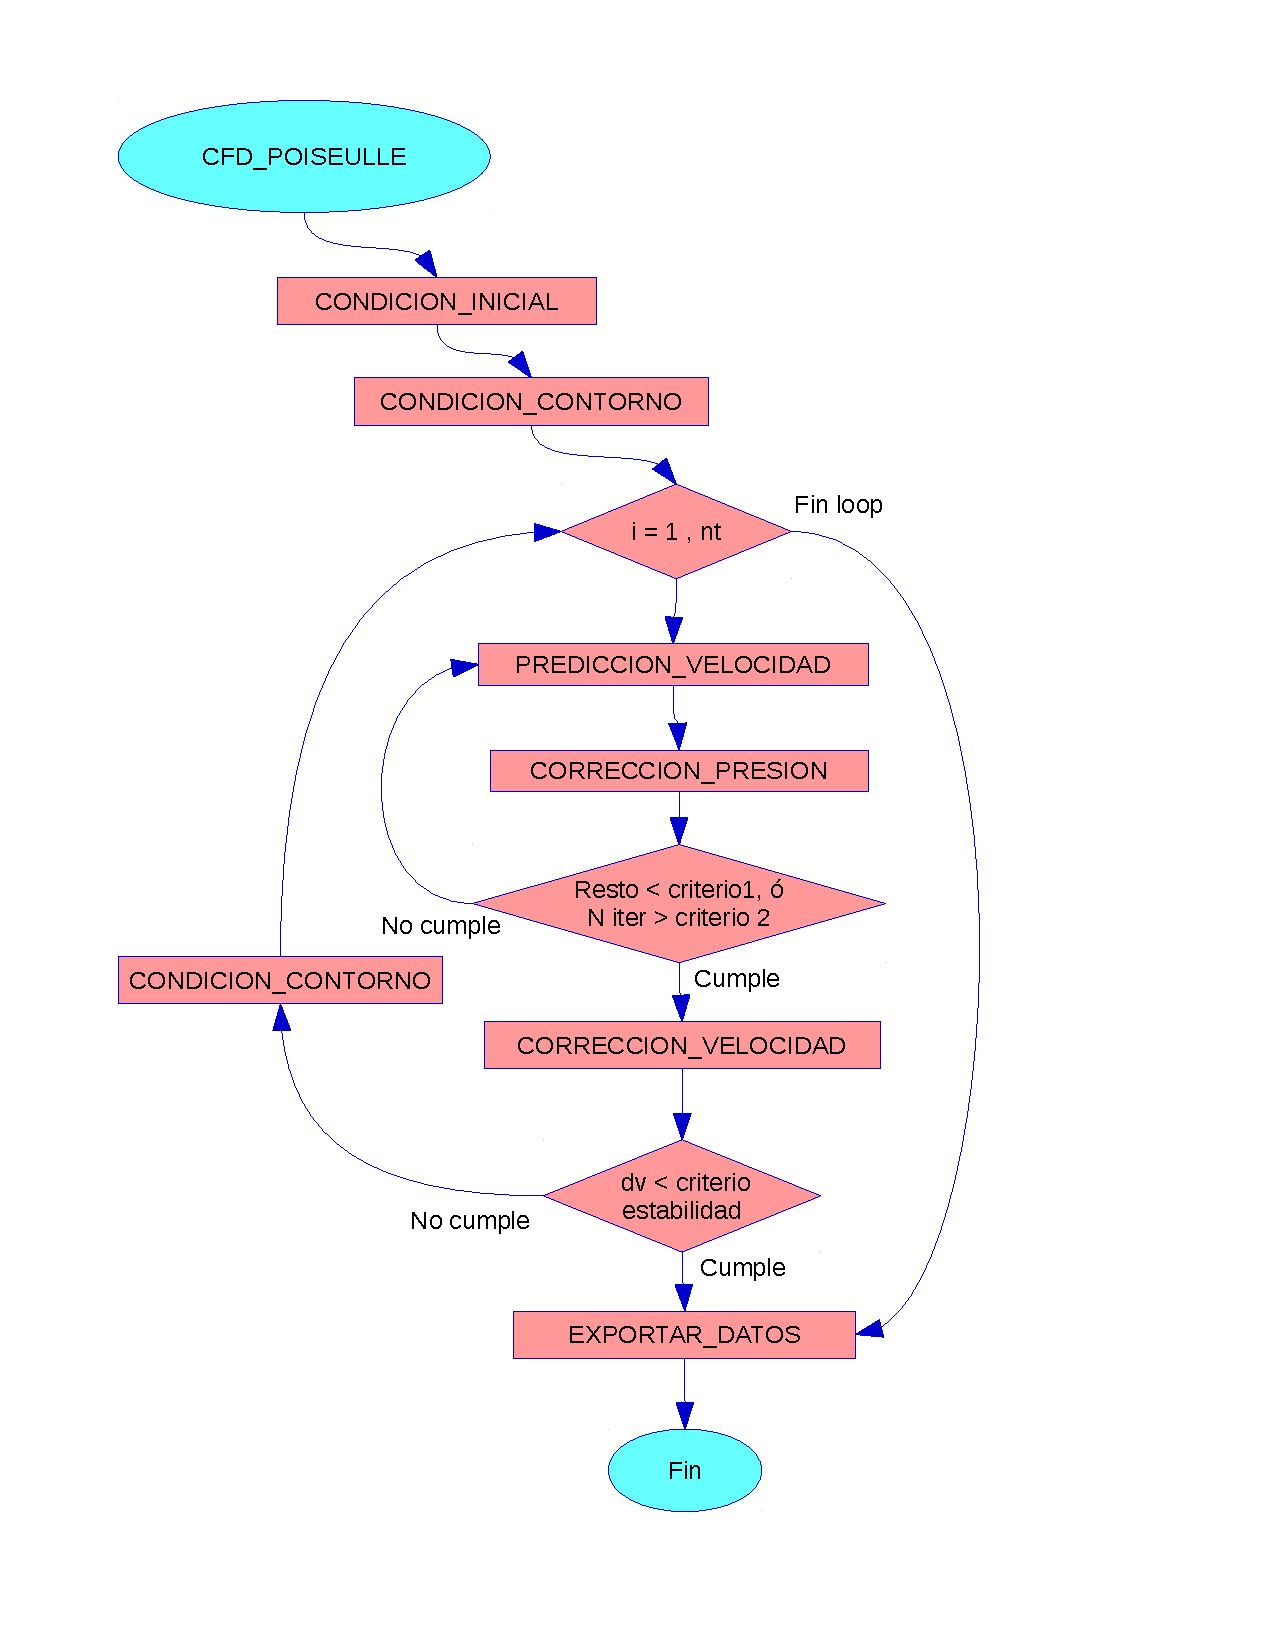
\includegraphics[width=1\textwidth]{diagrama_flujo_1.pdf}
\caption{Algoritmo de resolución para el problema de Poiseuille} \label{algoritmo}
\end{figure}
\end{center}

\paragraph{Condiciones de contorno} Establece condición de no deslizamiento en la cara inferior (i=2,j) y simetría en la cara superior (i=ny+1,j). 

\subparagraph{Condición de entrada y salida} Se plantean dos alternativas de resolución
\begin{itemize}
\item Se imponen condición de presión en la entrada y salida de la tubería, de tal manera de poder calcular directamente $\Delta P$ y poder comparar el perfil de velocidad con la solución analítica de Poiseuille.
\item Se imponen condición periódica para obtener el perfil desarrollado
\end{itemize}

\newpage
%---------------------------------------------

\section{Resultados}

Se muestra a continuación los resultados numéricos obtenidos. En la Figuras \ref{fig_1} y \ref{fig_2} se muestra el campo de velocidad y de presión de la mitad inferior de la tubería.  En la Figura \ref{fig_3} se comparar los resultados de perfil de velocidad en $x=Lx/2$ para modificando la razón de proporción de los volúmenes. En la medida que se vuelven menos regulares (alejandose de la relación 1:1, $Lx=5$, $nx=50$, $Ly=1$, $ny=10$) los resultados se alejan de la solución analítica. \\

En la Tabla \ref{resultados_1} se determinan los número CFL que aseguran la estabilidad. Notar CFL disminuye en la medida que Re disminuye.

\begin{table}[H]
\centering
\begin{tabular}{|l|lll|} \hline
Re & 2000	& 1500	& 1000 \\
CFL & 0.30	& 0.23	& 0.15 \\
T[s] & 18.908	& 45.036 & 19.840 \\ \hline
\end{tabular}
\caption{Número CFL que asegura la convergencia para cada Re ($Lx=5$, $Ly=1$, $Nx=50$, $Ny=10$)} \label{resultados_1}
\end{table}


\begin{figure}[H]
\centering
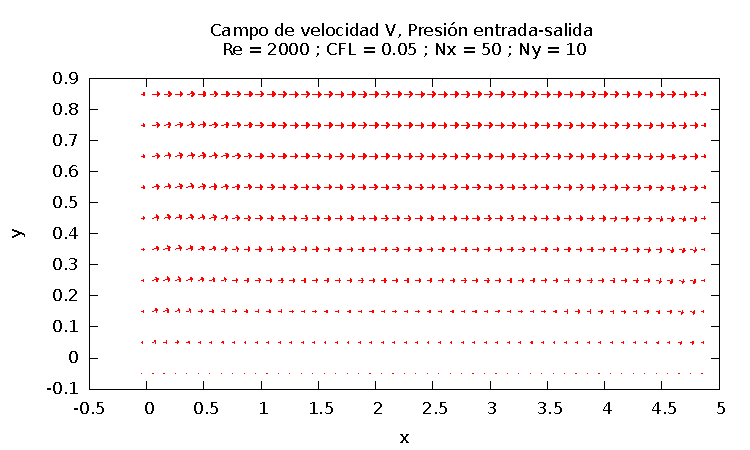
\includegraphics[width=1\textwidth]{./fig1_1/fig1_1/velocity_field.pdf}
\caption{} \label{fig_1}
\end{figure}

\begin{figure} [H]
\centering
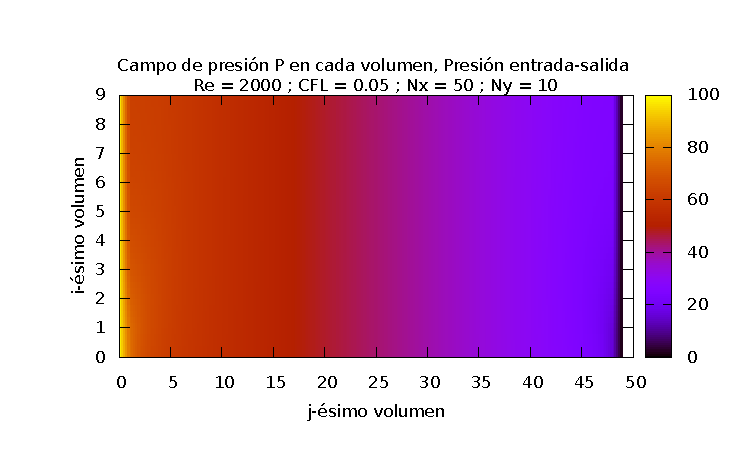
\includegraphics[width=1\textwidth]{./fig1_1/fig1_1/pressure_field.pdf}
\caption{} \label{fig_2}
\end{figure}

\begin{figure} [H]
\centering
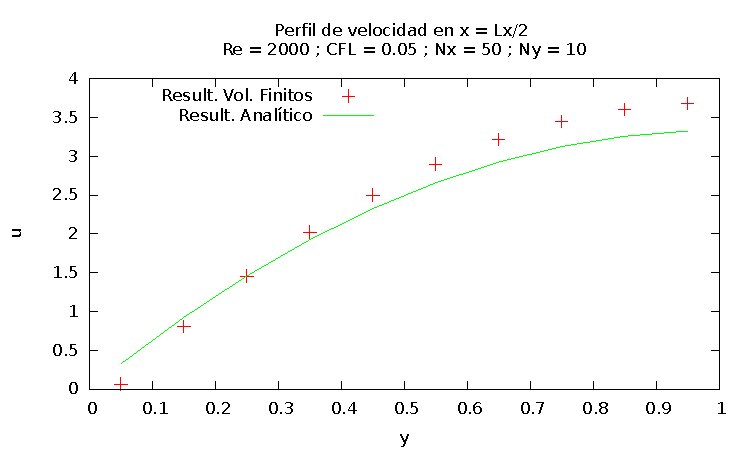
\includegraphics[width=0.8\textwidth]{./fig1_1/fig1_1/velocity_profile.pdf}
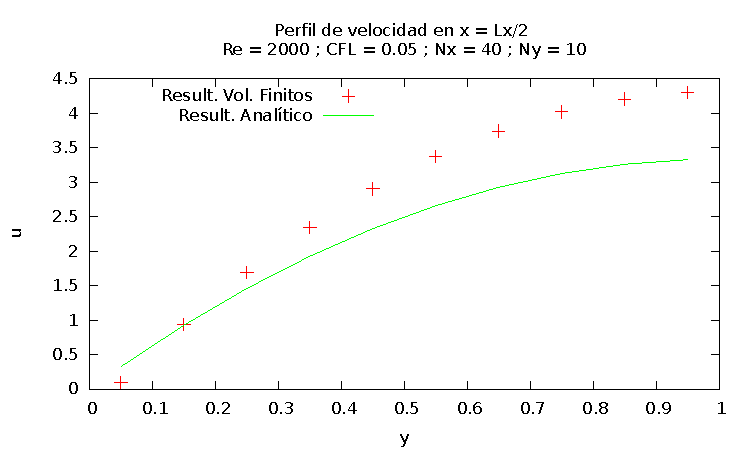
\includegraphics[width=0.8\textwidth]{./fig1_1/fig1_2/velocity_profile.pdf}
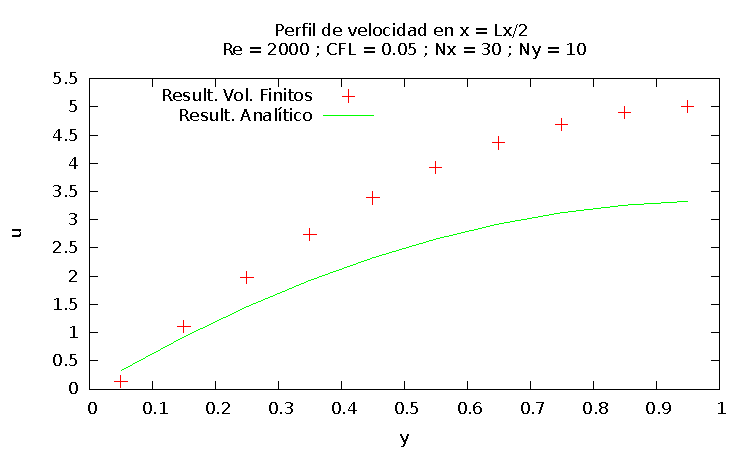
\includegraphics[width=0.8\textwidth]{./fig1_1/fig1_3/velocity_profile.pdf}
\caption{} \label{fig_3}
\end{figure}

\newpage
%---------------------------------------------

%\section{Conclusiones}

Los resultados números se contrastaron con los resultados analíticos del perfil de velocidad de un fluido incompresible viscoso que fluye en una tubería de sección circular. \\

Se comparan los resultados al imponer dos tipos de condición de contorno para la entrada y salida: Imposición de presión y flujo periódico. Se observa que para la condición de flujo periódico se obtiene un perfil con componente vertical prácticamente nulo, miestras que para la condición de presión existen componentes considerables en esta dirección. \\

Sin embargo utilizando esta condición se observa que se acerca más al perfil parabólico teórico que en el caso de flujo periodico. De está manera se puede ver cómo el problema presenta una sensibilidad a la elección de esta condición. Los tiempo de cálculo empleado con la condición periódica son mayores que las de la condición de presión: a ver las animaciones del flujo se observa que este \textit{oscila} a lo largo del tubo hasta lograr ser estacionario. Estos cambios repentinos requieren de rápidos cambios en la presión, por lo que se requieren de más iteraciones (en este caso, iteraciones de $\phi$) para lograr la convergencia de las variables. \\ 

El valor obtenido en la presión en ambos casos distan con creces, lo cual no tiene mayor relevancia al momento de resolver las ecuaciones que gobiernan al fluido ya que lo que influye es el gradiente de presión y no la presión en sí.\\

En la resolución de la ecuación de Poisson se utilizó una simplificación del operador laplaciano de $\phi$: Se omiten los valores vecinos del valor central. De esta manera se evita imponer condición de contorno para dicha variable, ya que se entiende que la presión es una función implícita de la velocidad, por lo que al imponer condición en la velocidad se imponen implícitamente para la presión. Sin embargo como se pudo apreciar, el resultado depende fuertemente de la condición de contorno, por lo que intentar otra aproximación de esta operación puede mejorar los resultados. \\

%\newpage
%---------------------------------------------

\begin{thebibliography}{3}

\bibitem{patankar} \textsc{Patankar, .S.} , \textit{Numerical Heat Transfer and Fluid Flow, (Series in computational methods in mechanics and thermal sciences)}, Taylor \& Francis, ISBN 0-89116-522-3

\bibitem{versteeg} \textsc{Versteeg, H., Malalasekera, W.,} , \textit{An introduction to Computational Fluid Dynamics}, John Wiley \& Sons Inc., 1995, ISBN 0-582-21884-5

\bibitem{ferz} \textsc{Ferziger, J., Peric, M.,} , \textit{Computational Methods for Fluid Dynamics}, Springer, 2002, ISBN 3-540-42074-6

\bibitem{liu} \textsc{Liu, G., R.,} , \textit{Meshfree Methods: Moving Beyond the Finite Element Method}, CRC Press ,2010, ISBN 978-1-4200-8209-8


\end{thebibliography}

\end{document}